% Created 2015-08-06 Thu 16:35
\documentclass[presentation]{beamer}
\usepackage[utf8]{inputenc}
\usepackage[T1]{fontenc}
\usepackage{fixltx2e}
\usepackage{graphicx}
\usepackage{longtable}
\usepackage{float}
\usepackage{wrapfig}
\usepackage{rotating}
\usepackage[normalem]{ulem}
\usepackage{amsmath}
\usepackage{textcomp}
\usepackage{marvosym}
\usepackage{wasysym}
\usepackage{amssymb}
\usepackage{hyperref}
\tolerance=1000
\usepackage{minted}
\usepackage{multirow}
\usepackage{minted}
\usepackage{fontspec}
\usepackage{graphicx}
\usepackage{subcaption}
\newminted{ruby}{fontsize=\scriptsize}
\usepackage{./theme/beamerthemeCristian}
\usepackage[nocolor]{./theme/beamerAlvinMacros}
\usepackage[absolute,overlay]{textpos}
\setlength{\TPHorizModule}{\paperwidth}
\setlength{\TPVertModule}{\paperheight}
\textblockorigin{0mm}{0mm}
\usepackage{natbib}
\usepackage{bibentry}
\usepackage{dirtree}
\newcommand\Fontvi{\fontsize{6}{7.2}\selectfont}
\nobibliography*
\usepackage{appendixnumberbeamer}
\usetheme{default}
\usecolortheme{}
\usefonttheme{}
\useinnertheme{}
\useoutertheme{}
\author{Cristian Ruiz, Emmanuel Jeanvoine and Lucas Nussbaum \\ \vspace{0.5cm} INRIA Nancy, France}
\date{}
\title{Performance Evaluation of Containers for HPC}
\hypersetup{
  pdfkeywords={},
  pdfsubject={},
  pdfcreator={Emacs 24.3.1 (Org mode 8.2.10)}}
\begin{document}




\sloppy
\frame{
  \thispagestyle{empty}
  \titlepage
  \begin{center}
    \includegraphics[height=1.2cm]{logos/inr_logo_sans_sign_coul.png}
    \hspace{0.5cm}
  \insertlogo{\includegraphics[height=1.2cm]{logos/grid5000.png}}
   \hspace{0.5cm}
  \insertlogo{\includegraphics[height=1.2cm]{logos/logo_loria_complet_couleur.pdf}}
  \end{center}

}

\tableofcontents



\section{Introduction}
\label{sec-1}

{\setbeamercolor{background canvas}{bg=basicallyblack}
\usebeamercolor[fg]{inverted text}
\begin{frame}[label=sec-1-1]{Linux Containers}


\par {\usebeamerfont{title} Container based virtualization}\par
\vspace{1cm} %\hfill
\end{frame}
}


\begin{frame}[label=sec-1-2]{Containers}
\begin{itemize}
\item \alert{Containers} refers generally to \alert{Operating-system-level virtualization},
where the \alert{kernel} of an operating system allows for multiple isolated \alert{user-space instances}.
\end{itemize}

\begin{figure}[!h]
  \center
  \includegraphics[scale=0.65]{figures/lxc-vm.jpg}
  \label{fig:hpc}
\end{figure}
\end{frame}

\begin{frame}[label=sec-1-3]{Implementations}
\begin{itemize}
\item Chroot
\item Linux-VServer
\item FreeBSD Jails
\item Solaris Containers
\item OpenVZ
\item Linux-Containers (LXC)
\end{itemize}
\end{frame}

\begin{frame}[label=sec-1-4]{\emph{namesapces and cgroups}}
Both features incorporated in Linux kenerl since 2006 (Linux 2.6.24).
Several container solutions: LXC, Docker, libcontainer, systemd-nspawn.

\begin{figure}[!h]
  \center
  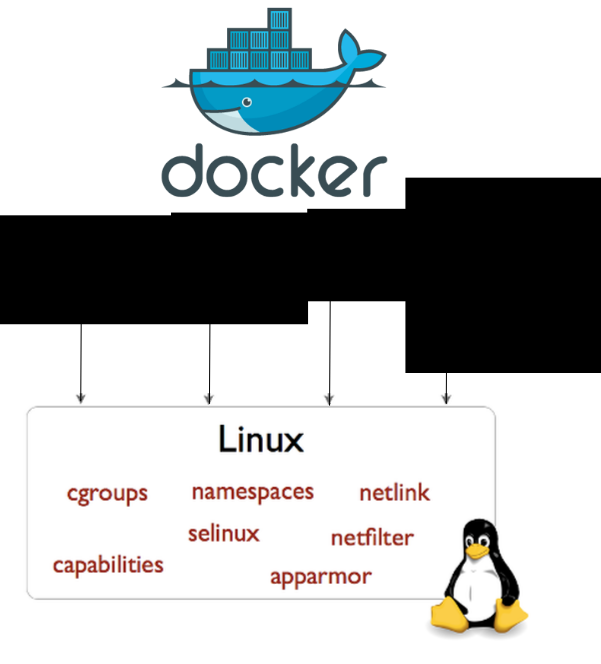
\includegraphics[scale=0.20]{figures/libcontainer-diagram.png}
  \label{fig:hpc}
\end{figure}

\emph{libcontainer} \alert{will become the standard to manage containers}
\end{frame}



\section{State of the art}
\label{sec-2}
\begin{frame}[label=sec-2-1]{Virtualization solutions for HPC}
\begin{itemize}
\item Youssef et al\cite{Youseff:2006:EPI:1308175.1308346} evaluated Xen using HPC
Challenge benczhmarks and LLNL ASC Purple benchmarks.

\item Nussbaum et al\cite{nussbaum2009linux} compared Xen and KVM using
micro-benchmarks and the HPC Challenge benchmarks.

\item Regola et al\cite{regola2010recommendations} focuses on the I/O
performance of Xen, KVM and OpenVZ.

\item Public Cloud platforms: Amazon EC2 \cite{5353067} and Microsoft Azure\cite{Tudoran:2012:PEA:2168697.2168701}
  have been evaluated using Intel MPI benchmarks and scientific applications.
\end{itemize}
\end{frame}

\begin{frame}[label=sec-2-2]{Container performance evaluation}
\begin{itemize}
\item Matthews et al\cite{matthews2007quantifying} compared the performance of VMWare,
Xen, Solaris containers and OpenVZ using custom benchmarks.
\item Felter et al\cite{ibmtrdocker} evaluated the I/O performance of Docker using MySQL
Linpack, Stream, RandomAccess, nuttcp, netperf, fio, and Redis.
\item Walter et al\cite{4482796} compared VMWare Server, Xen and OpenVZ using NetPerf, IOZone, and the NAS Parallel Benchmarks.

\item Xavier et al\cite{6498558} compared Linux VServer, OpenVZ,
LXC and Xen using the HPC Challenge benchmarks and the NAS
Parallel Benchmarks.
\end{itemize}
\end{frame}

{\setbeamercolor{background canvas}{bg=basicallyblack}
\usebeamercolor[fg]{inverted text}
\begin{frame}[label=sec-2-3]{In this work, we answer:}



\begin{itemize}
\item What is the overhead of oversubscription using different versions of Linux kernel?
\item What is the performance of inter-container communication?
\item What is the impact of moving an HPC workload with several MPI processes per machine, to containers?
\item Our experimental setup included up to 64 machines.
\end{itemize}
\end{frame}
}



\section{Experimental evaluation}
\label{sec-3}

\begin{frame}[label=sec-3-1]{Experimental setup}
\begin{block}{Hardware}
Cluster in Grid'5000 Testbed\cite{grid5000} where each node is equipped with two Intel Xeon E5-2630v3 processors (with 8 cores each), 128 GB of RAM and
a 10 Gigabit Ethernet adapter.
\end{block}

\begin{block}{Software}
Debian Jessie, Linux kernel versions: 3.2, 3.16 and 4.0, TAU version 2.23.1, OpenMPI version 1.6.5 and NPB version 3.3.
We wrote recipes\footnote{https://github.com/camilo1729/distem-recipes} to install the necessary software using
Kameleon\cite{Ruiz:2015:RSA:2723872.2723883}.

We instrumented the benchmarks: LU, EP, CG, MG, FT, IS using TAU\cite{Shende06thetau}.
\end{block}
\end{frame}

\begin{frame}[label=sec-3-2]{Linux kernel version}
\begin{figure}[!h]
  \center
  \includegraphics[scale=0.40]{figures/execution_time-kernel-cgB.pdf}
  \label{fig:hpc}
\end{figure}
\end{frame}

\begin{frame}[label=sec-3-3]{Oversubscription}
\begin{figure}[!h]
  \center
  \includegraphics[scale=0.40]{figures/execution_time-tso-40.pdf}
  \label{fig:hpc}
\end{figure}
\end{frame}


\begin{frame}[label=sec-3-4]{Linux kernel version and oversubscription}
\begin{itemize}
\item Overall, we observed a maximum performance gain of around 77\%
when passing from 3.2 to 3.16 and 11\% when passing form 3.16 to 4.0.

\item Regarding Linux 4.0, there is not significant difference between running 1 or 2 container per physical machine.
\end{itemize}
\end{frame}

\begin{frame}[label=sec-3-5]{Inter-container communication}
\begin{itemize}
\item 1 physical node: \emph{container} and \emph{SM}
\item 8 physical nodes: \emph{native}
\end{itemize}

All running the equivalent number of MPI processes.

\begin{figure}[H]
  \centering
\begin{subfigure}[b]{0.42\textwidth}
    \includegraphics[scale=0.25,angle=0]{figures/inter-container-mgC.pdf}
    \caption{CG Class B}
  \end{subfigure}
  \begin{subfigure}[b]{0.42\textwidth}
    \includegraphics[scale=0.25,angle=0]{figures/inter-container-isC.pdf}
    \caption{IS Class C}
  \end{subfigure}
\end{figure}
\end{frame}

\begin{frame}[label=sec-3-6]{Inter-container communication}
\begin{itemize}
\item Although inter-container communication is faster
than communication among physical machines, there is an important degradation
of the CPU performance for applications that are memory bound.

\item Virtual network device does not add an extra cost.
\end{itemize}
\end{frame}

\begin{frame}[label=sec-3-7]{Multinode inter-container communication}
\begin{itemize}
\item 16 MPI processes were run per physical machine or container
\item We used a maximum of 32 physical machines.
\end{itemize}

\begin{figure}
  \centering
  \begin{subfigure}[b]{0.42\textwidth}
    \includegraphics[scale=0.25,angle=0]{figures/veth_overhead-tso-cgB.pdf}
    \caption{CG Class B}
  \end{subfigure}
  \begin{subfigure}[b]{0.42\textwidth}
    \includegraphics[scale=0.25,angle=0]{figures/veth_overhead-tso-ftB.pdf}
    \caption{FT Class B}
  \end{subfigure}
\end{figure}
\end{frame}

\section{Conclusions}
\label{sec-4}
\section{Bibliography}
\label{sec-5}
\begin{frame}[label=sec-5-1]{Bibliography}

\bibliography{distem_validation.bib}
\bibliographystyle{plain}
\appendix
\end{frame}
% Emacs 24.3.1 (Org mode 8.2.10)
\end{document}
